% ----------------------------------------------------
% Experimentation
% ----------------------------------------------------
\documentclass[class=report,11pt,crop=false]{standalone}
\input{../Style/ChapterStyle.tex}
\makenoidxglossaries
% --------------------------------------------------------------------
% Examples of creating a glossary
\newacronym{cw}{CW}{Continuous-Wave}
\newacronym{dsp}{DSP}{Digital Signal Processing}
\newacronym{em}{EM}{Electromagnetic}
\newacronym{fmcw}{FMCW}{Frequency Modulated Continuous Wave}
\newacronym{gui}{GUI}{Graphical User Interface}
\newacronym{rf}{RF}{Radio Frequency}
\newacronym{radar}{RADAR}{Radio Detection and Ranging}
\newacronym{pcb}{PCB}{Printed Circuit Board}
\newacronym{pc}{PC}{Personal Computer}
\newacronym{pri}{PRI}{Pulse Repetition Interval}
\newacronym{adc}{ADC}{Analogue-to-Digital Converter}
\newacronym{if}{IF}{Intermediate Frequency}
\newacronym{itu}{ITU}{International Telecommunications Union}
\newacronym{rcs}{RCS}{Radar Cross Section}
\newacronym{opamp}{Op Amp}{Operational Amplifier}
\newacronym{gbwp}{GBWP}{Gain Bandwidth Product}
\newacronym{dc}{DC}{Direct Current}
\newacronym{ac}{AC}{Alternating Current}
\newacronym{uct}{UCT}{University of Cape Town}
\newacronym{usb}{USB}{Universal Serial Bus}
\newacronym{stft}{STFT}{Short-Time Fourier Transform}
\newacronym{fft}{FFT}{Fast Fourier Transform}
\newacronym{dft}{DFT}{Discrete Fourier Transform}
\newacronym{dtft}{DTFT}{Discrete-Time Fourier Transform}
\newacronym{snr}{SNR}{Signal-to-Noise Ratio}
\newacronym{prf}{PRF}{Pulse Repetition Frequency}
\newacronym{isar}{ISAR}{Inverse Synthetic Aperture}
% include SUV (check experimentation table)
% --------------------------------------------------------------------

\begin{document}
% ----------------------------------------------------
\chapter{Experimentation \label{ch:experimentation}}
\vspace{-1cm}
% ----------------------------------------------------
\section{Equipment and tools}
The equipment and tools used to conduct the experiments are as follows:
\begin{itemize}
    \item Two desks
    \item Two chairs
    \item Laptop
    \item External sound card (XONAR U5)
    \item Demonstrator in enclosure
    \item Measuring tape
    \item Notebook and pencil
    \item Paper and tape for distance markings
    \item Cellphone
    \item Reflective vests
\end{itemize}

For safety, reflective vests were worn and the relevant security in the area were informed of the experiments being conducted; permission was also granted when conducting experiments in a public area such as a mall or apartment building.

\section{Experimental Setup}
The experiments were conducted in indoor and outdoor parking areas to evaluate the performance of the demonstrator in various conditions and environments. To perform these experiments, the demonstrator had to be placed in a convenient and effective position for the detection of the vehicles. Figure~\ref{fig:setup} shows the setup used which included the enclosed demonstrator, \gls{pc}, and external sound card. 

% Experimental setup
\begin{figure}[htbp]
    \centering
    \captionsetup{type=figure}
    \begin{subfigure}[t]{0.5\textwidth}
        \centering
        \def\svgwidth{1\linewidth}
        {\scriptsize
            \setstretch{0.7} % Line spacing
            \includegraphics[width=6cm,height=6cm]{../Images/experimental_setup.drawio.png}}
        \caption{Experimental setup diagram.}
        \label{fig:setup-diagram}
    \end{subfigure}
    ~ 
    \begin{subfigure}[t]{0.4\textwidth}
        \def\svgwidth{1\linewidth}
        {\scriptsize
            \setstretch{0.7} % Line spacing
            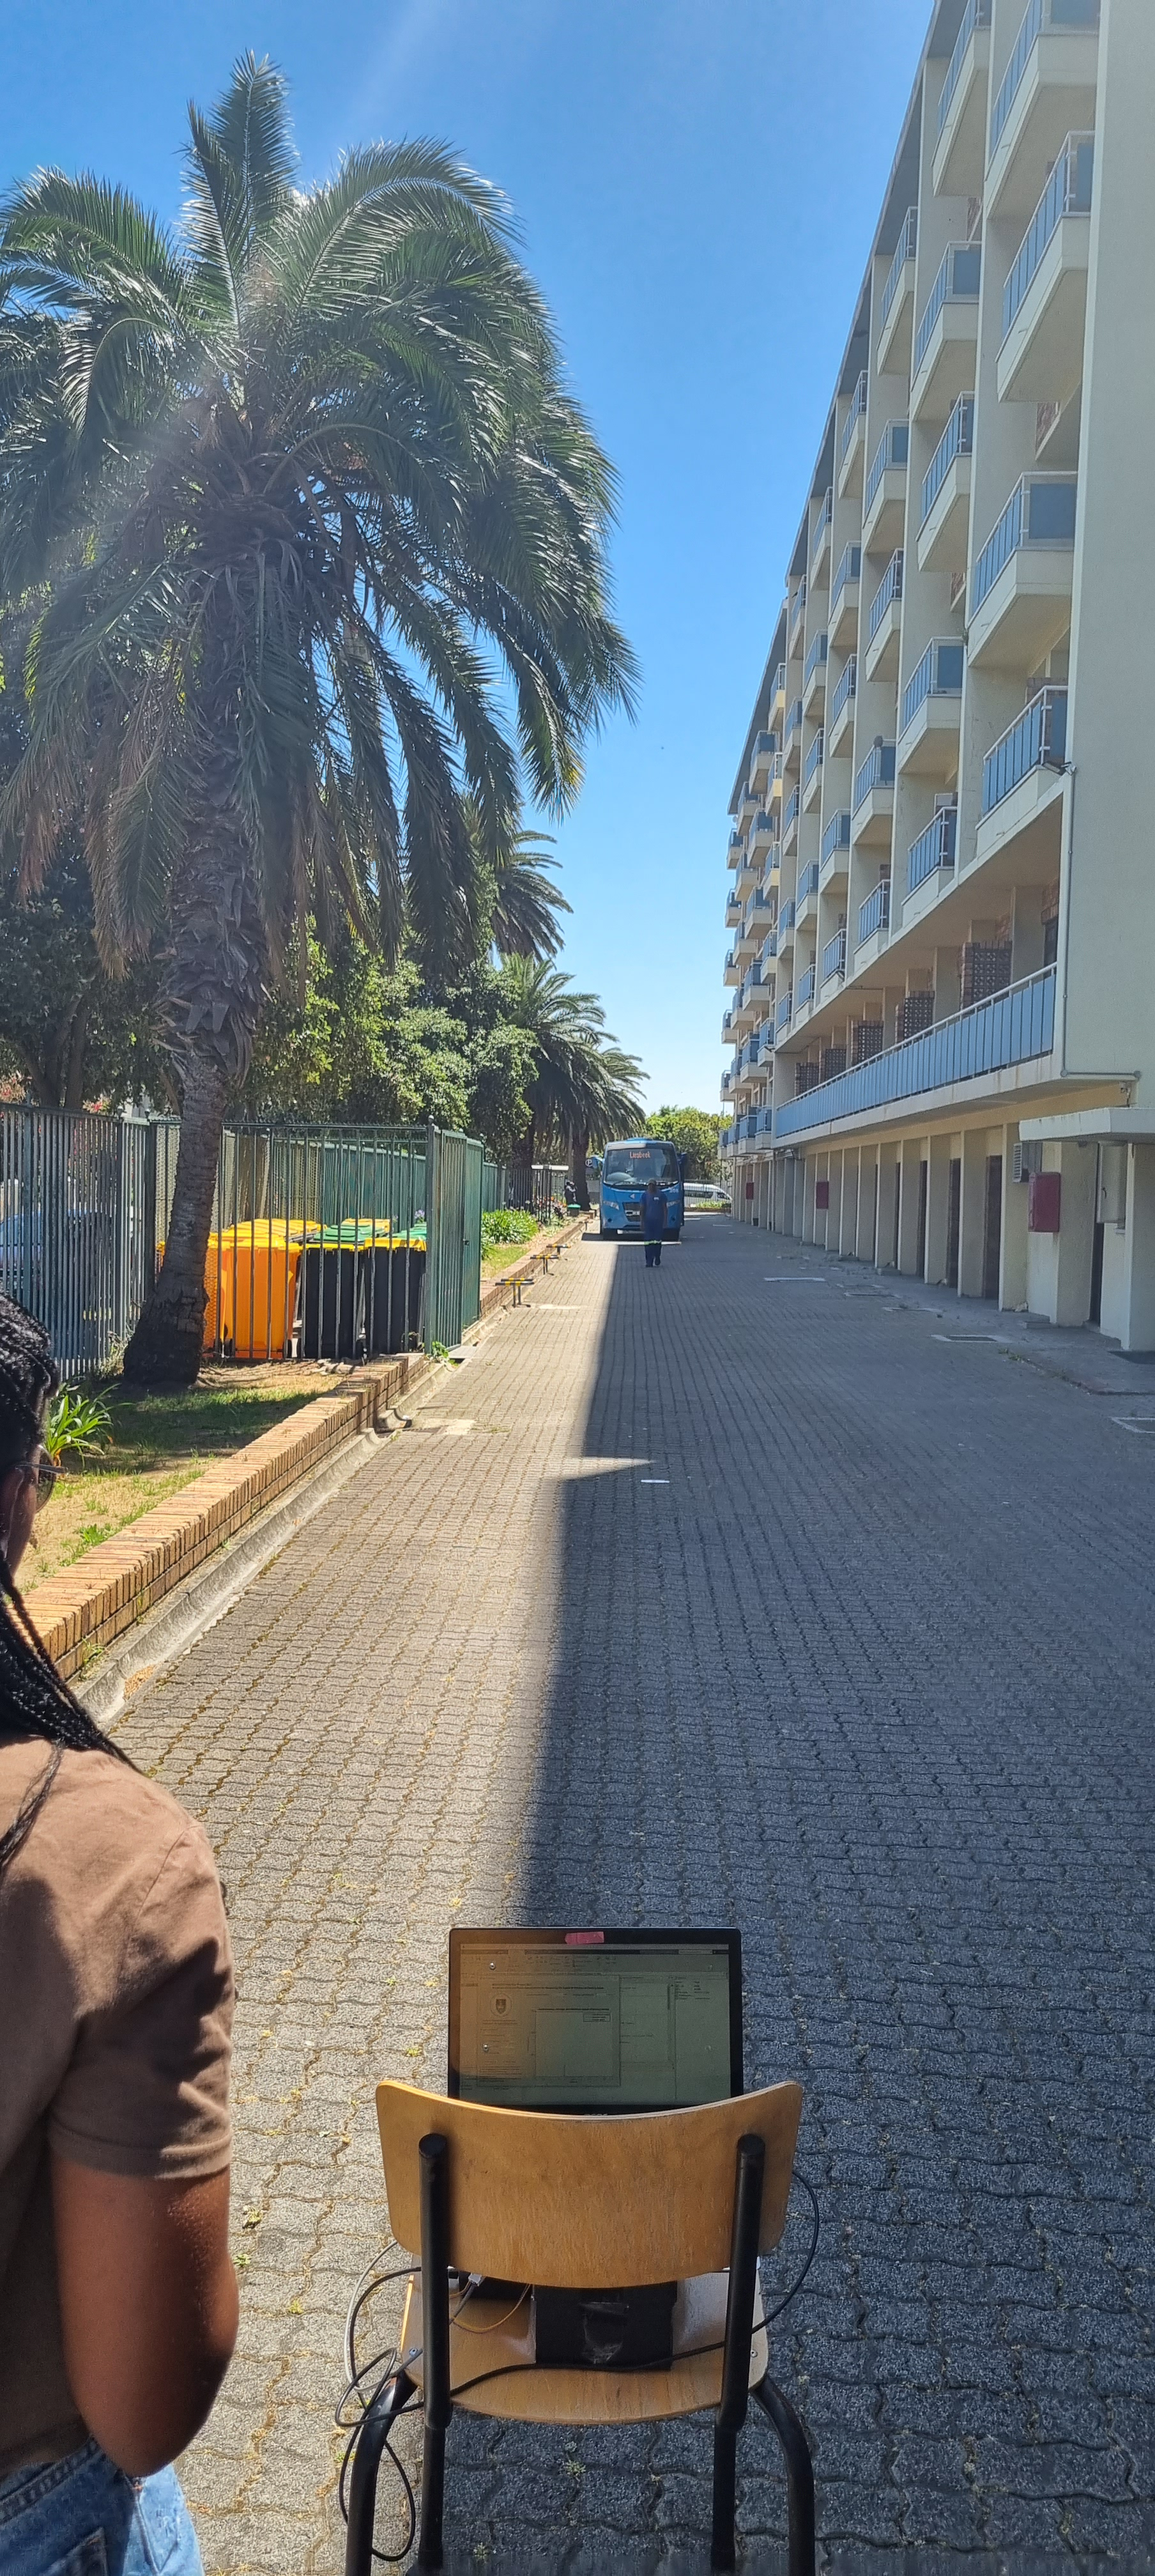
\includegraphics[width=6.5cm,height=6cm]{../Images/setup_outdoor.png}}
        \caption{Setup of demonstrator in outdoor parking area.}
        \label{fig:setup-outdoor}
    \end{subfigure}
    ~
    \begin{subfigure}[t]{0.5\textwidth}
        \centering
        \def\svgwidth{1\linewidth}
        {\scriptsize
            \setstretch{0.7} % Line spacing
            \includegraphics[width=6cm,height=6cm]{../Images/setup_indoor.png}}
        \caption{Point-of-view of demonstrator in indoor parking area.}
        \label{fig:setup-indoor}
    \end{subfigure}
    \caption{Experimental setup.}
    \label{fig:setup}
\end{figure}

For experiments conducted in non-ideal areas, the demonstrator, sound card, and \gls{pc} were held with the demonstrator being level to the moving vehicle.

\section{Experiments}
\subsection{Speed}\label{subsect:speed}
This experiment was conducted to determine if the demonstrator could pick up the speed of the moving vehicles up to 20 km/h. Once the demonstrator is setup, the algorithm is run from the \textsc{MATLAB} application (the design is explained in Section~\ref{sect:gui}) which displays the instantaneous, average, and maximum speeds of the vehicle in question. This data is saved to a \textbf{\textsc{.mat}} file and tabulated in the report. To validate the speed displayed on the \textsc{MATLAB} \gls{gui}, a video is recorded and the speed is determined using Equation~\ref{eqn:speed}. Where possible, the driver is asked to give the speed that the vehicle was moving at and this information is tabulated as well.

\begin{equation}
    Speed = \frac{Distance}{Time}
    \label{eqn:speed}
\end{equation}

The distance is taken from the time the car moves past one distance marking until it crosses the ground marking point. The difference between the time stamps at these markings is used in Equation~\ref{eqn:speed}. At least three vehicles are used for this experiment.

\subsection{Range}\label{subsect:range}
This experiment evaluates the demonstrator's range of detection. As shown in Figure~\ref{fig:setup-diagram}, distance markings are placed on the floor between the demonstrator and target vehicle. When the car is in position, the \textsc{MATLAB} application begins logging just before the car passes the marking and is run for 5 s at a time. Distance markings are placed at 5 m, 10 m, and 15 m. Equation~\ref{eqn:range} is then used to determine the range of the radar for each vehicle.

% re-evaluate this section
\subsection{Vehicle Size}
The \gls{rcs} is a measure of how detectable the vehicle is by the ultrasonic radar. The purpose of this experiment is to determine the maximum size of vehicle that the radar is able to detect and is conducted similarly to that in Section~\ref{subsect:speed} and Section~\ref{subsect:range}. The cross-sectional area of the vehicle is then used to make a comment on the calculated \gls{rcs} of the target vehicle. Table~\ref{tab:vehicle-sizes} shows the standard measurements of three vehicles of different sizes used in this experiment. Small-to-medium sized cars include small cars (also known as city cars), small SUVs, and mid-size cars (for four-door vehicles). Bus dimensitons are taken for small and large single-deck busses.

\begin{table}[!htp]
\centering
\caption{\label{tab:vehicle-sizes} Standard measurements of three vehicles of different sizes}
\vspace{-0.5cm}
\begin{tabular}{|m{10em}|m{3cm}|m{3cm}|m{3cm}|}
\multicolumn{4}{l}{}\\
\cline{1-4}
Vehicle             &   Width (m)    &   Length (m)   &   Height (m)    \\ \cline{1-4}
Motorcycle          & 0.635 to 1.016 &  1.905 to 2.54 &  1.016 to 1.524 \\ \cline{1-4}
Small-to-medium car & 1.475 to 1.871 &  2.7 to 4.73   &  1.46 to 1.61   \\ \cline{1-4}
Bus                 &     2.85       &   10 to 13.5   &     3.4          \\ \cline{1-4}
\end{tabular}
\end{table}

% ----------------------------------------------------
\ifstandalone
\bibliography{../Bibliography/References.bib}
\printnoidxglossary[type=\acronymtype,nonumberlist]
\fi
\end{document}
% ----------------------------------------------------